\documentclass[12pt]{article}

\usepackage[paperheight=3.5in,paperwidth=4in,top=.25in,bottom=0in,right=0in,left=0in]{geometry}
%fancy math symbols
\usepackage{amsmath}
\usepackage{amssymb}
\usepackage{cancel}
%fancy font
%\usepackage{pxfonts}
\usepackage[T1]{fontenc}
%DAGs
\usepackage{tikz}
\usetikzlibrary{arrows,positioning,snakes,calc,shapes}
\tikzset{>=latex}
\usepackage{subfig}
\captionsetup[subfloat]{position = top, font = large} % For sub-figure captions
\renewcommand{\thesubfigure}{\normalsize\Alph{subfigure})}
\usepackage{float}

\begin{document}
\begin{figure}[H]
\begin{center}
\captionsetup[subfigure]{oneside,margin={-4cm,0cm},labelformat=simple,labelsep=period}

\subfloat[]{
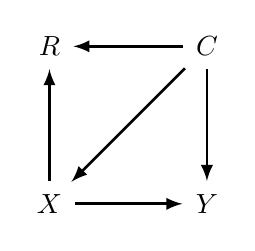
\begin{tikzpicture}[line width=1pt]

\node [align=center] (x) at (0,0) {$X$};
\node [align=center] (r) at (0,2) {$R$};
\node [align=center] (y) at (2,0) {$Y$};
\node [align=center] (c) at (2,2) {$C$};

\begin{scope}[line width=1pt,shorten >= 1pt, shorten <= 1pt]
\draw[->,color=black] (x) to (r);
\draw[->,color=black] (x) to (y);
\draw[->,color=black] (c) to (r);
\draw[->,color=black] (c) to (x);
\draw[->,color=black] (c) to (y);
\end{scope}

\end{tikzpicture}
}
\subfloat[]{
\hspace{2cm}
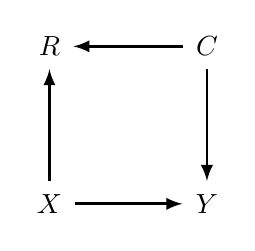
\begin{tikzpicture}[line width=1pt]

\node [align=center] (x) at (0,0) {$X$};
\node [align=center] (r) at (0,2) {$R$};
\node [align=center] (y) at (2,0) {$Y$};
\node [align=center] (c) at (2,2) {$C$};

\begin{scope}[line width=1pt,shorten >= 1pt, shorten <= 1pt]
\draw[->,color=black] (x) to (r);
\draw[->,color=black] (x) to (y);
\draw[->,color=black] (c) to (r);
%\draw[->,color=black] (c) to (x);
\draw[->,color=black] (c) to (y);
\end{scope}

\end{tikzpicture}
}

\subfloat[]{
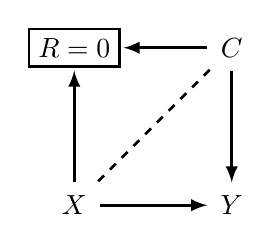
\begin{tikzpicture}[line width=1pt]

\node [align=center] (x) at (0,0) {$X$};
\node [align=center,draw] (r) at (0,2) {$R=0$};
\node [align=center] (y) at (2,0) {$Y$};
\node [align=center] (c) at (2,2) {$C$};

\begin{scope}[line width=1pt,shorten >= 1pt, shorten <= 1pt]
\draw[->,color=black] (x) to (r);
\draw[->,color=black] (x) to (y);
\draw[->,color=black] (c) to (r);
\draw[-,color=black,dashed] (c) to (x);
\draw[->,color=black] (c) to (y);
\end{scope}

\end{tikzpicture}
}
\subfloat[]{
\hspace{2cm}
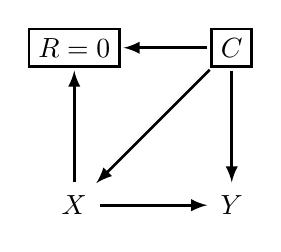
\begin{tikzpicture}[line width=1pt]

\node [align=center] (x) at (0,0) {$X$};
\node [align=center,draw] (r) at (0,2) {$R=0$};
\node [align=center] (y) at (2,0) {$Y$};
\node [align=center,draw] (c) at (2,2) {$C$};

\begin{scope}[line width=1pt,shorten >= 1pt, shorten <= 1pt]
\draw[->,color=black] (x) to (r);
\draw[->,color=black] (x) to (y);
\draw[->,color=black] (c) to (r);
\draw[->,color=black] (c) to (x);
\draw[->,color=black] (c) to (y);
\end{scope}

\end{tikzpicture}
}
\end{center}
\end{figure}
\end{document}